\section{\ruby{質問}{しつもん}フォーム}
わからないこと、\ruby{質問}{しつもん}したいことがあれば\ruby{質問}{しつもん}フォームから\ruby{質問}{しつもん}しよう!

\ruby{質問}{しつもん}フォームでは、\ruby{授業}{じゅぎょう}でわからなかったことや\ruby{確認}{かくにん}したいことなどをホームページを通して\ruby{質問}{しつもん}できます。
たくさん\ruby{質問}{しつもん}してわからないことを\ruby{解決}{かいけつ}しよう。

1.
ブラウザで\textbf{\ruby{授業}{じゅぎょう}で使うホームページリスト}を開こう。

\textbf{\ruby{授業}{じゅぎょう}で使うホームページリスト}は01フォルダの中のlinks.htmlです

リストの4番目の子ども\textbf{IT\ruby{未来塾}{みらいじゅく}\ruby{質問}{しつもん}フォーム}をクリックして開いてください(図~\ref{fig:51})。


\bigskip

{\bfseries
  スマートフォン等からの場合は\url{https://bit.ly/2NHiVgi}を開いてください。}



\centering
\begin{figure}[H]
  \begin{minipage}{\textwidth}
    {\upshape
      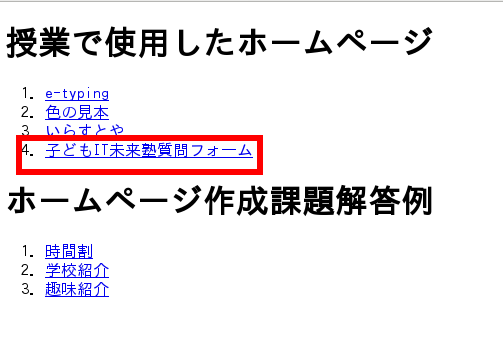
\includegraphics[width=0.9\textwidth]{text01-img/textbook-img245.png}
      \caption{ホームページリストより\ruby{質問}{しつもん}フォームを開く}\label{fig:51}
    }
  \end{minipage}  
\end{figure}


\bigskip

\bigskip
\clearpage
2.
\ruby{質問}{しつもん}フォーム(図~\ref{fig:52})が\ruby{表示}{ひょうじ}されます

\centering
\begin{figure}[H]
  \begin{minipage}{\textwidth}
    {\upshape
      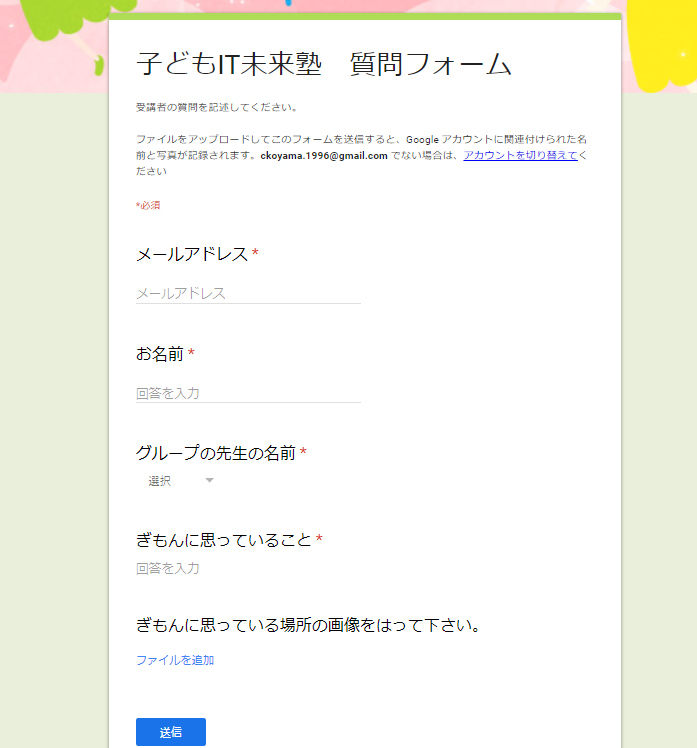
\includegraphics[width=0.7\textwidth]{text01-img/textbook-img246.png}
      \caption{\ruby{質問}{しつもん}フォーム}\label{fig:52}
    }
  \end{minipage}  
\end{figure}

\flushleft

\bigskip

メールアドレス、お名前、グループの先生の名前、ぎもんに思っていることを入力します。
必要に\ruby{応}{おう}じて、ぎもんに思っている場所の\ruby{画像}{がぞう}を追加してください。

{\bfseries
送信\textmd{を\ruby{押}{お}すと\ruby{質問}{しつもん}ができます。図~\ref{fig:53}の画面が出たら\ruby{質問}{しつもん}は\ruby{完了}{かんりょう}です。}}



\centering
\begin{figure}[H]
  \begin{minipage}{\textwidth}
    {\upshape
      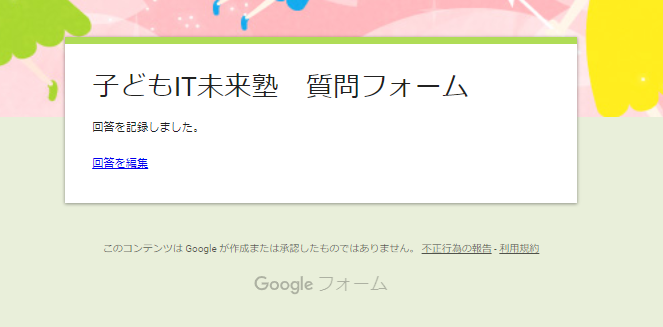
\includegraphics[width=0.45\textwidth]{text01-img/textbook-img247.png}
      \caption{\ruby{質問}{しつもん}送信画面}\label{fig:53}
    }
  \end{minipage}  
\end{figure}

\flushleft
メールアドレスのらんに入力したアドレスへグループの先生から回答メールがきます。
メールが来るまで、しばらくお待ちください。数日かかる場合があります。

